\newpage
\section{Gestione questionari}
Selezionata la voce \textit{Gestione questionari} dal menù a sinistra il sistema visualizza la seguente pagina, dalla quale un utente può gestire i propri questionari:

\label{GestioneQuestionari}
\begin{figure}[ht]
	\centering
	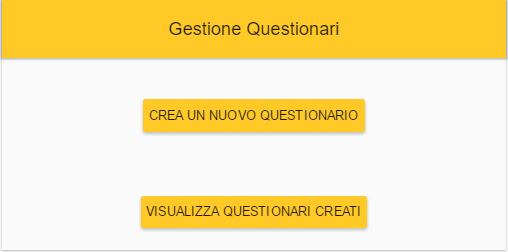
\includegraphics[scale=0.55]{img/gestione_questionari.png}
	\caption{Gestione questionari}
\end{figure}
\FloatBarrier

\subsection{Crea un nuovo questionario}
Selezionando la voce \textit{CREA UN NUOVO QUESTIONARIO} si avvia la funzionalità di creazione di un questionario:

\label{CreazioneQuestionari}
\begin{figure}[ht]
	\centering
	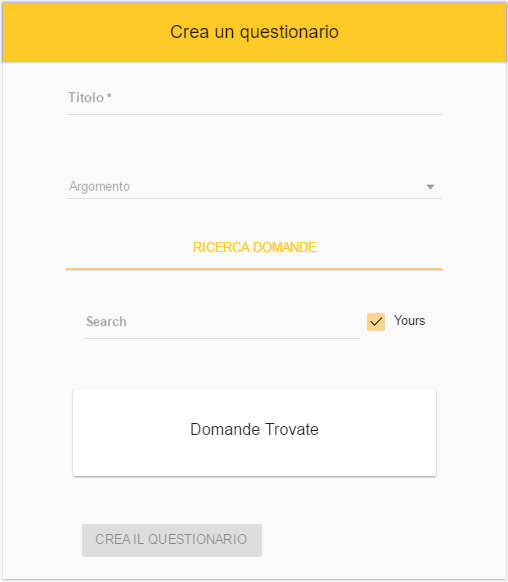
\includegraphics[scale=0.55]{img/creazione_questionario.png}
	\caption{Creazione questionario}
\end{figure}
\FloatBarrier

Sara possibile scegliere un \textit{Titolo} e un \textit{Argomento} da associare al questionario che si sta creando. In più si potranno inserire le domande ricercandole tra le proprie create oppure all'interno del sistema, digitando le parole chiave associate. Compilati tutti i campi dati necessari il bottone \textit{CREA IL QUESTIONARIO} viene abilitato e permetterà di creare il questionario. 

\subsection{Visualizza questionari creati}
Selezionando la voce \textit{VISUALIZZA QUESTIONARI CREATI} è possibile visualizzare i propri questionari:

\label{VisualizzaQuestionari}
\begin{figure}[ht]
	\centering
	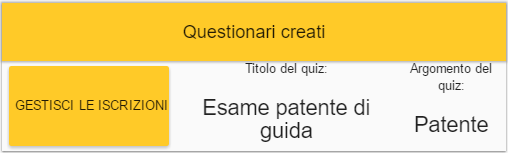
\includegraphics[scale=0.55]{img/visualizza_questionari.png}
	\caption{Visualizza questionari}
\end{figure}
\FloatBarrier

A fianco del titolo di ogni questionario compare un bottone che porta alla gestione delle iscrizioni al proprio questionario creato. Si potrà dunque decidere chi, tra gli utenti richiedenti l'iscrizione, abilitare e chi no.
